% Created by tikzDevice version 0.12.6 on 2025-11-06 14:23:27
% !TEX encoding = UTF-8 Unicode
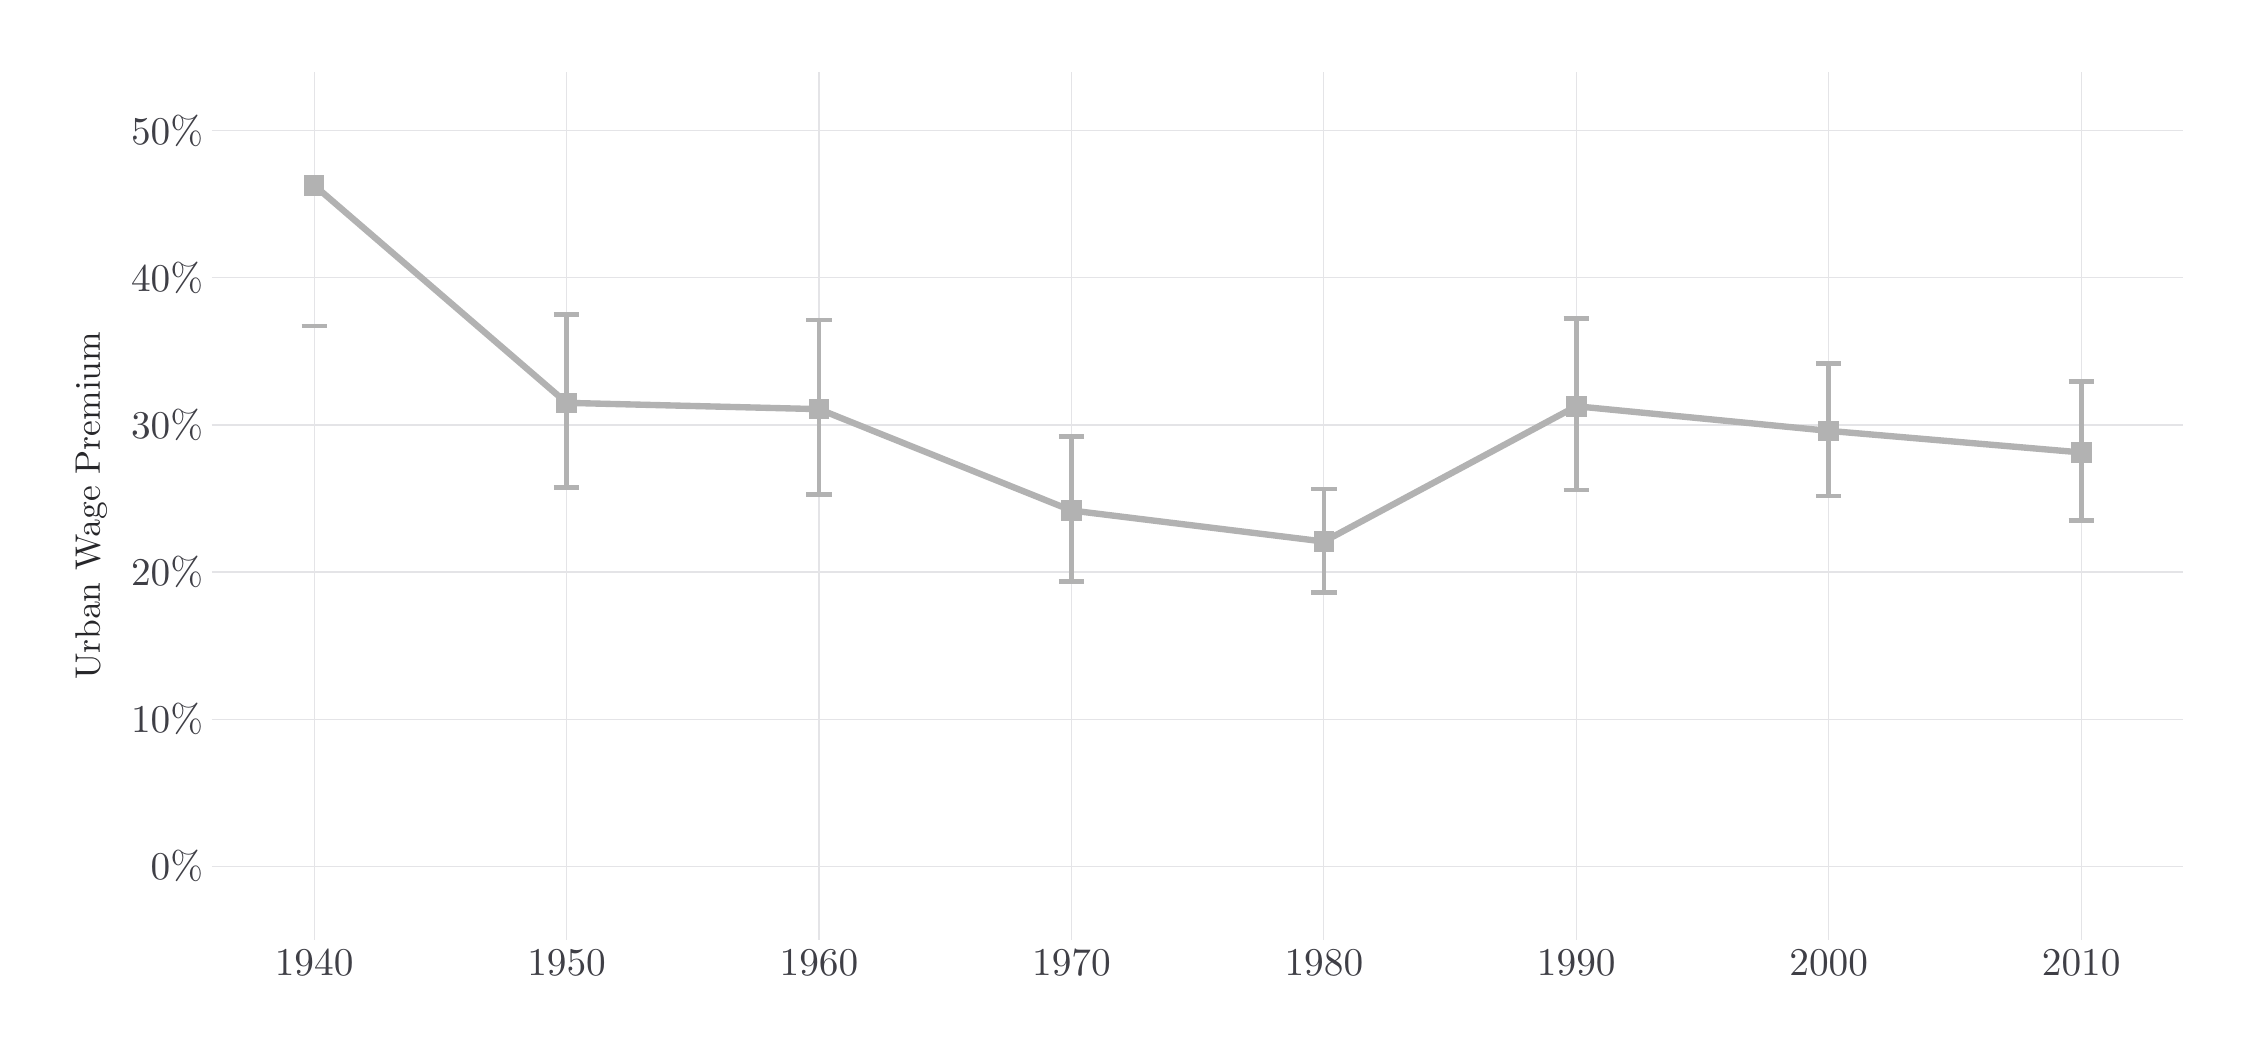
\begin{tikzpicture}[x=1pt,y=1pt]
\definecolor{fillColor}{RGB}{255,255,255}
\path[use as bounding box,fill=fillColor] (0,0) rectangle (794.97,361.35);
\begin{scope}
\path[clip] (  0.00,  0.00) rectangle (794.97,361.35);
\definecolor{drawColor}{RGB}{255,255,255}

\path[draw=drawColor,line width= 0.8pt,line join=round,line cap=round,fill=fillColor] (  0.00,  0.00) rectangle (794.97,361.35);
\end{scope}
\begin{scope}
\path[clip] ( 66.57, 31.76) rectangle (778.97,345.35);
\definecolor{drawColor}{RGB}{255,255,255}
\definecolor{fillColor}{RGB}{255,255,255}

\path[draw=drawColor,line width= 0.8pt,line join=round,line cap=round,fill=fillColor] ( 66.57, 31.76) rectangle (778.97,345.35);
\definecolor{drawColor}{RGB}{228,228,231}

\path[draw=drawColor,line width= 0.4pt,line join=round] ( 66.57, 58.33) --
	(778.97, 58.33);

\path[draw=drawColor,line width= 0.4pt,line join=round] ( 66.57,111.48) --
	(778.97,111.48);

\path[draw=drawColor,line width= 0.4pt,line join=round] ( 66.57,164.64) --
	(778.97,164.64);

\path[draw=drawColor,line width= 0.4pt,line join=round] ( 66.57,217.79) --
	(778.97,217.79);

\path[draw=drawColor,line width= 0.4pt,line join=round] ( 66.57,270.94) --
	(778.97,270.94);

\path[draw=drawColor,line width= 0.4pt,line join=round] ( 66.57,324.09) --
	(778.97,324.09);

\path[draw=drawColor,line width= 0.4pt,line join=round] (103.51, 31.76) --
	(103.51,345.35);

\path[draw=drawColor,line width= 0.4pt,line join=round] (194.73, 31.76) --
	(194.73,345.35);

\path[draw=drawColor,line width= 0.4pt,line join=round] (285.94, 31.76) --
	(285.94,345.35);

\path[draw=drawColor,line width= 0.4pt,line join=round] (377.16, 31.76) --
	(377.16,345.35);

\path[draw=drawColor,line width= 0.4pt,line join=round] (468.38, 31.76) --
	(468.38,345.35);

\path[draw=drawColor,line width= 0.4pt,line join=round] (559.59, 31.76) --
	(559.59,345.35);

\path[draw=drawColor,line width= 0.4pt,line join=round] (650.81, 31.76) --
	(650.81,345.35);

\path[draw=drawColor,line width= 0.4pt,line join=round] (742.03, 31.76) --
	(742.03,345.35);
\definecolor{drawColor}{gray}{0.70}

\path[draw=drawColor,line width= 2.3pt,line join=round] (103.51,304.41) --
	(194.73,225.78) --
	(285.94,223.50) --
	(377.16,186.88) --
	(468.38,175.66) --
	(559.59,224.55) --
	(650.81,215.66) --
	(742.03,207.86);

\path[draw=drawColor,line width= 1.7pt,line join=round] ( 98.95,253.53) --
	(108.07,253.53);

\path[draw=drawColor,line width= 1.7pt,line join=round] (190.17,257.71) --
	(199.29,257.71);

\path[draw=drawColor,line width= 1.7pt,line join=round] (194.73,257.71) --
	(194.73,195.24);

\path[draw=drawColor,line width= 1.7pt,line join=round] (190.17,195.24) --
	(199.29,195.24);

\path[draw=drawColor,line width= 1.7pt,line join=round] (281.38,255.72) --
	(290.50,255.72);

\path[draw=drawColor,line width= 1.7pt,line join=round] (285.94,255.72) --
	(285.94,192.70);

\path[draw=drawColor,line width= 1.7pt,line join=round] (281.38,192.70) --
	(290.50,192.70);

\path[draw=drawColor,line width= 1.7pt,line join=round] (372.60,213.66) --
	(381.72,213.66);

\path[draw=drawColor,line width= 1.7pt,line join=round] (377.16,213.66) --
	(377.16,161.15);

\path[draw=drawColor,line width= 1.7pt,line join=round] (372.60,161.15) --
	(381.72,161.15);

\path[draw=drawColor,line width= 1.7pt,line join=round] (463.82,194.61) --
	(472.94,194.61);

\path[draw=drawColor,line width= 1.7pt,line join=round] (468.38,194.61) --
	(468.38,157.25);

\path[draw=drawColor,line width= 1.7pt,line join=round] (463.82,157.25) --
	(472.94,157.25);

\path[draw=drawColor,line width= 1.7pt,line join=round] (555.03,256.21) --
	(564.15,256.21);

\path[draw=drawColor,line width= 1.7pt,line join=round] (559.59,256.21) --
	(559.59,194.26);

\path[draw=drawColor,line width= 1.7pt,line join=round] (555.03,194.26) --
	(564.15,194.26);

\path[draw=drawColor,line width= 1.7pt,line join=round] (646.25,239.99) --
	(655.37,239.99);

\path[draw=drawColor,line width= 1.7pt,line join=round] (650.81,239.99) --
	(650.81,192.16);

\path[draw=drawColor,line width= 1.7pt,line join=round] (646.25,192.16) --
	(655.37,192.16);

\path[draw=drawColor,line width= 1.7pt,line join=round] (737.47,233.51) --
	(746.59,233.51);

\path[draw=drawColor,line width= 1.7pt,line join=round] (742.03,233.51) --
	(742.03,183.15);

\path[draw=drawColor,line width= 1.7pt,line join=round] (737.47,183.15) --
	(746.59,183.15);
\definecolor{fillColor}{gray}{0.70}

\path[fill=fillColor] ( 99.78,300.68) --
	(107.24,300.68) --
	(107.24,308.14) --
	( 99.78,308.14) --
	cycle;

\path[fill=fillColor] (191.00,222.05) --
	(198.46,222.05) --
	(198.46,229.51) --
	(191.00,229.51) --
	cycle;

\path[fill=fillColor] (282.21,219.77) --
	(289.67,219.77) --
	(289.67,227.23) --
	(282.21,227.23) --
	cycle;

\path[fill=fillColor] (373.43,183.15) --
	(380.89,183.15) --
	(380.89,190.61) --
	(373.43,190.61) --
	cycle;

\path[fill=fillColor] (464.65,171.93) --
	(472.11,171.93) --
	(472.11,179.39) --
	(464.65,179.39) --
	cycle;

\path[fill=fillColor] (555.86,220.82) --
	(563.32,220.82) --
	(563.32,228.28) --
	(555.86,228.28) --
	cycle;

\path[fill=fillColor] (647.08,211.93) --
	(654.54,211.93) --
	(654.54,219.39) --
	(647.08,219.39) --
	cycle;

\path[fill=fillColor] (738.30,204.13) --
	(745.76,204.13) --
	(745.76,211.59) --
	(738.30,211.59) --
	cycle;
\end{scope}
\begin{scope}
\path[clip] (  0.00,  0.00) rectangle (794.97,361.35);
\definecolor{drawColor}{RGB}{63,63,70}

\node[text=drawColor,anchor=base east,inner sep=0pt, outer sep=0pt, scale=  1.42] at ( 63.37, 53.44) {0\%};

\node[text=drawColor,anchor=base east,inner sep=0pt, outer sep=0pt, scale=  1.42] at ( 63.37,106.59) {10\%};

\node[text=drawColor,anchor=base east,inner sep=0pt, outer sep=0pt, scale=  1.42] at ( 63.37,159.74) {20\%};

\node[text=drawColor,anchor=base east,inner sep=0pt, outer sep=0pt, scale=  1.42] at ( 63.37,212.89) {30\%};

\node[text=drawColor,anchor=base east,inner sep=0pt, outer sep=0pt, scale=  1.42] at ( 63.37,266.04) {40\%};

\node[text=drawColor,anchor=base east,inner sep=0pt, outer sep=0pt, scale=  1.42] at ( 63.37,319.19) {50\%};
\end{scope}
\begin{scope}
\path[clip] (  0.00,  0.00) rectangle (794.97,361.35);
\definecolor{drawColor}{RGB}{63,63,70}

\node[text=drawColor,anchor=base,inner sep=0pt, outer sep=0pt, scale=  1.42] at (103.51, 18.76) {1940};

\node[text=drawColor,anchor=base,inner sep=0pt, outer sep=0pt, scale=  1.42] at (194.73, 18.76) {1950};

\node[text=drawColor,anchor=base,inner sep=0pt, outer sep=0pt, scale=  1.42] at (285.94, 18.76) {1960};

\node[text=drawColor,anchor=base,inner sep=0pt, outer sep=0pt, scale=  1.42] at (377.16, 18.76) {1970};

\node[text=drawColor,anchor=base,inner sep=0pt, outer sep=0pt, scale=  1.42] at (468.38, 18.76) {1980};

\node[text=drawColor,anchor=base,inner sep=0pt, outer sep=0pt, scale=  1.42] at (559.59, 18.76) {1990};

\node[text=drawColor,anchor=base,inner sep=0pt, outer sep=0pt, scale=  1.42] at (650.81, 18.76) {2000};

\node[text=drawColor,anchor=base,inner sep=0pt, outer sep=0pt, scale=  1.42] at (742.03, 18.76) {2010};
\end{scope}
\begin{scope}
\path[clip] (  0.00,  0.00) rectangle (794.97,361.35);
\definecolor{drawColor}{RGB}{39,39,42}

\node[text=drawColor,rotate= 90.00,anchor=base,inner sep=0pt, outer sep=0pt, scale=  1.28] at ( 26.06,188.55) {Urban Wage Premium};
\end{scope}
\end{tikzpicture}
